% --- Block 3 divider (from sections/diffusion/stable-diffusion-lecture/block3-extra.tex) ---
\section{Latent Diffusion and Stable Diffusion}

% \begin{frame}{Perceptual vs.\ semantic compression}
%   Pixel-space diffusion is redundant: the U-Net spends capacity on imperceptible high-frequency detail.
%   \textbf{Stable Diffusion} (Rombach et al., 2022) decouples:
%   \begin{enumerate}
%     \item \textbf{Perceptual compression (VAE):} $\mathcal{E}: \mathbf{x} \mapsto \mathbf{z}$---remove imperceptible spatial detail; preserve layout.
%     \item \textbf{Semantic generation (LDM):} run diffusion on $\mathbf{z}$---lower memory, faster training.
%     \item \textbf{Decode:} $\mathcal{D}(\mathbf{z}) \mapsto \mathbf{x}$---project back to pixels.
%   \end{enumerate}
%   Typical spatial downsampling: $8\times$ (e.g., $512 \times 512 \rightarrow 64 \times 64$ latents).
% \end{frame}

% \begin{frame}{Cross-attention: injecting text into the U-Net}
%   \textbf{Pipeline:} CLIP text encoder $\rightarrow$ token embeddings $\mathbf{c} \in \mathbb{R}^{L \times d}$.
%   \begin{itemize}
%     \item \textbf{Self-attention:} Q, K, V from spatial latent features---global visual coherence.
%     \item \textbf{Cross-attention:} Q from spatial features; K, V from text embeddings---align patches with prompt tokens.
%   \end{itemize}
%   \[
%     \mathrm{Attention}(Q, K, V) = \mathrm{softmax}\!\left(\frac{QK^\top}{\sqrt{d_k}}\right) V
%   \]
%   Scaling by $\sqrt{d_k}$ prevents softmax saturation in high dimensions.
%   \footnotesize Token length $L \leq 77$ (CLIP); multi-head attention throughout U-Net ResNet blocks.
% \end{frame}

% --- Latent diffusion (from sections/diffusion/complete/latent-diffusion.tex) ---
\section{Latent Diffusion Models (LDMs)}
\begin{frame}{}
    \LARGE Stable Diffusion: \textbf{A Latent Diffusion Model (LDM)}
\end{frame}

\begin{frame}[allowframebreaks]{What is a Latent Space?}
    \begin{figure}
        \centering
        \fetchconvertimage{https://nvlabs.github.io/LSGM/assets/pipelinefig.png}{images/diffusion/latent-space-diffusion.png}{width=\textwidth,height=0.5\textheight,keepaspectratio}
    \end{figure}
    \begin{itemize}
        \setlength{\itemsep}{-0.5em}
        \item A \textbf{latent space} is an abstract, compressed space where high-dimensional data (like images) is represented in a lower-dimensional form.
        \item Think of it as a hidden layer of meaning—each point in this space represents a potential image or concept.
        \item In classical models like GANs or VAEs, the latent space is directly sampled from (e.g., a vector $\mathbf{z}$), and the generator turns it into an image.
        \item \textbf{Latent} space = ``Hidden space of ideas or features''
    \end{itemize}
\end{frame}

\begin{frame}{Where is the Latent Space in Diffusion?}
    \textbf{Two main ways latent spaces are used in diffusion:}
    \begin{itemize}
        \item \textbf{1. Latent Diffusion Models (LDMs):}
        \begin{itemize}
            \item Diffusion is performed in a compressed latent space, not directly on high-dimensional images.
            \item \textbf{Pipeline:} Compress image $\rightarrow$ Denoise in latent space $\rightarrow$ Decode back to image.
            \item Enables faster, cheaper training and inference, and allows for semantic control (e.g., text prompts, masks).
        \end{itemize}
        \item \textbf{2. Latent Representations in Noise Vectors:}
        \begin{itemize}
            \item Even in standard diffusion models, the initial noise vector acts as a latent code.
            \item Changing the noise vector generates different images or morphs between them.
        \end{itemize}
    \end{itemize}
\end{frame}

\begin{frame}{Why Latent Diffusion?}
    \begin{itemize}
        \item \textbf{Traditional pixel-space diffusion models are computationally expensive}: they operate directly on high-dimensional images, making both training and inference costly.
        \item \textbf{Latent diffusion reduces computational cost} by performing the diffusion process in a compressed, lower-dimensional latent space—while still maintaining high-quality image generation.
        \item This efficiency enables more complex and practical applications, such as text-guided generation and flexible image editing.
        \item \textbf{How is this achieved?} Instead of working in pixel space, we learn a compressed latent space using a Variational Autoencoder (VAE) with very low KL divergence weight (e.g., $10^{-6}$). This yields a compact representation suitable for diffusion.
        \item This approach mirrors ideas from autoregressive models (e.g., VQGAN), enabling even more efficient and controllable generation pipelines.
    \end{itemize}
\end{frame}

% \begin{frame}{Latent Diffusion Models (Stable Diffusion): Key Concepts}
%     \begin{itemize}
%         \item \textbf{Latent Diffusion Models (LDMs):} Operate in a compressed latent space for efficiency.
%         \item \textbf{Diffusion Process:} Gradually adds noise to data, then learns to reverse this process.
%         \item \textbf{Text Conditioning:} Uses CLIP text encoders to guide image generation from prompts.
%     \end{itemize}
% \end{frame}

% \begin{frame}{Latent Diffusion Models: Architecture Overview}
%     \textbf{Architecture Overview}
%     \begin{itemize}
%         \item \textbf{Encoder:} Maps images to latent space.
%         \item \textbf{UNet:} Core denoising network operating in latent space.
%         \item \textbf{Decoder:} Reconstructs images from latent representations.
%         \item \textbf{Text Encoder:} CLIP-based, encodes prompts for conditioning.
%     \end{itemize}
% \end{frame}

\begin{frame}{Latent Diffusion Models: Visual Overview}
    \begin{figure}
        \centering
        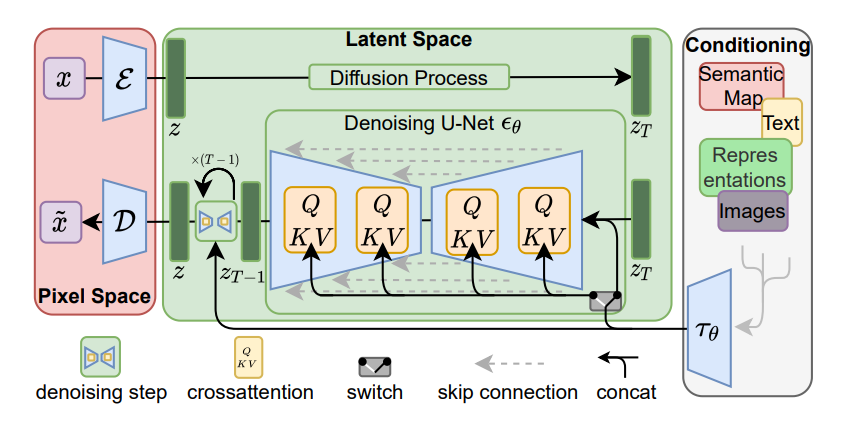
\includegraphics[width=1.05\linewidth,height=0.95\textheight,keepaspectratio]{images/adv-img-gen/slide_97_1_img.png}
    \end{figure}
\end{frame}

% \begin{frame}{Applications of Stable Diffusion}
%     \begin{itemize}
%         \item Text-to-image generation (e.g., Stable Diffusion) uses text embeddings in latent space.
%         \item Image editing by modifying specific parts of the latent.
%         \item Inversion: map a real image to latent, edit, then decode back.
%     \end{itemize}
% \end{frame}
